%%%%%%%%%%%%%%%%%%%%%%%%%%%%%%%%%%%%%%%%%%%%%%%%%%%%%%%%%%%%%%%%%%%%%%%%%%%%%%%%%%%%%%%%%%%%%%%%%%%%%%
%
%   Filename    : appendix_A.tex 
%
%   Description : This file is for including the Research Ethics Documents (delegated as Appendix A) 
%                 
%%%%%%%%%%%%%%%%%%%%%%%%%%%%%%%%%%%%%%%%%%%%%%%%%%%%%%%%%%%%%%%%%%%%%%%%%%%%%%%%%%%%%%%%%%%%%%%%%%%%%%

\chapter{Appendix}
\label{sec:appendixa}

\section{Ha.Zee Command Line Help}

\begin{figure}[h!]
	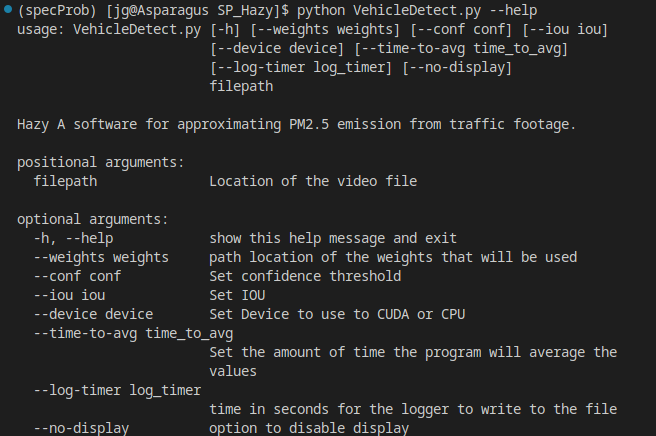
\includegraphics[width=\linewidth,scale=0.8]{ha_help.png}
	\caption{Ha.Zee command line help shown}
	\label{fig:cmd_help}
\end{figure}

Figure \ref{fig:cmd_help} shows the command line help for the “VehicleDetect” program. This helps the user to determine what the different arguments do and what is needed to run the program. This can be accessed via the terminal by inputting the command “python VehicleDetect.py -–help” or “python VehicleDetect.py -h”

\section{Log File}

\begin{figure}[h!]
	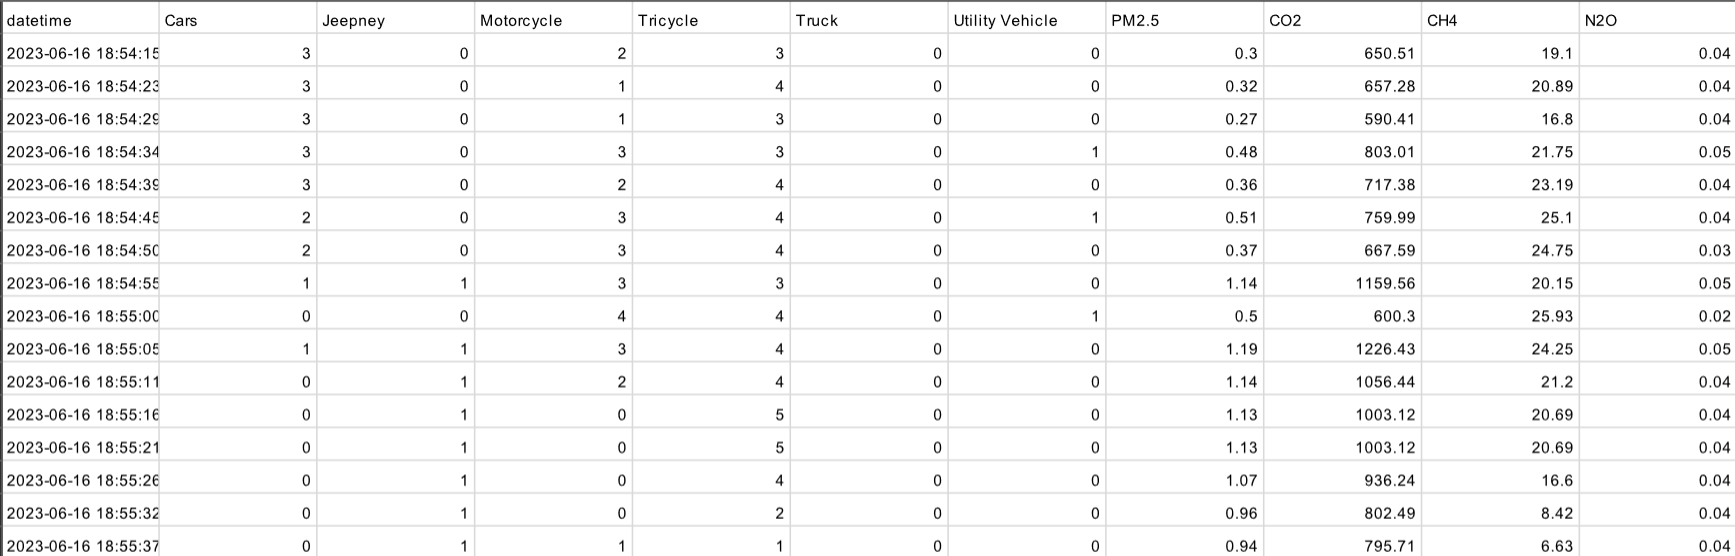
\includegraphics[width=\linewidth,scale=0.8]{logfile.png}
	\caption{Example Logfile where each entry was generated for approximately 5 seconds}
	\label{fig:logfile}
\end{figure}

To record the data, the results were saved in a CSV file as shown in Figure N.2. The recorded data was written using the current frame that it was recorded in, not the average, hence why the values on the recorded data vary a lot between time periods. 



% Save the file you want to include in PDF format.
% Uncomment the commant below specifying the correct appendix file. 
%\includepdf[pages=-, scale = 0.9, pagecommand={}, offset = -30 0]{appendixA.pdf}

